% !TEX program = lualatex
%==============================================================================
% プリアンブル (Preamble)
%==============================================================================

\documentclass[a4paper, 11pt]{ltjsarticle}

%------------------------------------------------------------------------------
% パッケージ読み込み
%------------------------------------------------------------------------------
\usepackage[margin=2.5cm]{geometry}
\usepackage{amsmath}           % 数式
\usepackage{booktabs}          % 表
\usepackage{siunitx}           % 単位
\usepackage{graphicx}          % 画像読み込み
\usepackage{float}             % 画像配置の制御
\usepackage{luatexja-fontspec} % 和文フォント
\usepackage{listings}          % ソースコード
\usepackage{xcolor}            % 色

% listings の設定
\lstset{
	basicstyle=\ttfamily\small,
	keywordstyle=\color{blue}\bfseries,
	commentstyle=\color{green!40!black},
	stringstyle=\color{red!60!black},
	numbers=left,
	numberstyle=\tiny,
	stepnumber=1,
	numbersep=5pt,
	frame=single,
	breaklines=true,
	breakatwhitespace=true,
	columns=fullflexible,
	showstringspaces=false,
	language=Python,
	inputencoding=utf8,
	captionpos=b
}

%------------------------------------------------------------------------------
% 各種設定
%------------------------------------------------------------------------------

% --- 和文フォント設定 ---
\setmainjfont[Renderer=HarfBuzz]{Yu Mincho}
\setsansjfont[Renderer=HarfBuzz]{Yu Gothic}

% --- ドキュメント情報 ---
\title{画像処理・画像処理工学 レポート課題1}
\author{画像処理工学科 学籍番号: 21239 組番号:234 5E 氏名:栁原 魁人}
\date{\today}

%==============================================================================
% ドキュメント本体 (Body)
%==============================================================================
\begin{document}

\maketitle
\thispagestyle{empty}
\clearpage

\section{課題1}

\subsection{問題1-1: メディアンカット量子化法}

\subsubsection{理論}
メディアンカット量子化法は、色空間を再帰的に分割することで、最適な代表色を決定する量子化手法です。元の画像の色数を削減しながら、画像の視覚的品質を維持します。

\textbf{基本原理:}
\begin{enumerate}
	\item カラーボックス(色の集合)で初期化
	\item ボックス内で最も分散が大きい色成分(R、G、B いずれか)を特定
	\item その成分の中央値で分割
	\item 目標の色数に達するまで繰り返す
	\item 各ボックスの平均色を代表色として確定
\end{enumerate}

\textbf{重要な点:}
\begin{itemize}
	\item 「最大分散軸」での分割により、色の多様性が高い方向を優先
	\item 「中央値」での分割により、各ボックス内のピクセル数がほぼ等しくなる
	\item 再帰的な処理で、色数の異なる多段階量子化が可能
\end{itemize}

\subsubsection{計算・導出過程}

図A-1に示す4×5画素の画像に対してメディアンカット量子化法を適用し、4色に量子化します。

\textbf{全ピクセル値の取得と整理:}

画像から抽出される全20ピクセルの値:
\begin{center}
	102, 179, 92, 14, 106, 74, 202, 87, 116, 99, 151, 130, 149, 52, 1, 235, 157, 37, 129, 191
\end{center}

\textbf{ステップ1: 全ピクセルをソートして4つのグループに分割}

全ピクセル値を昇順にソート:
\begin{center}
	1, 14, 37, 52, 74, 87, 92, 99, 102, 106, 116, 129, 130, 149, 151, 157, 179, 191, 202, 235
\end{center}

目標色数が4色なので、20個のピクセルを4つのグループに均等分割(各5ピクセル):

\begin{table}[H]
	\centering
	\caption{ピクセル値を4つのグループに均等分割}
	\begin{tabular}{|l|l|c|}
		\hline
		グループ & ピクセル値 & グループ内の位置 \\
		\hline
		グループ1 & 1, 14, 37, 52, 74 & 1~5番目 \\
		グループ2 & 87, 92, 99, 102, 106 & 6~10番目 \\
		グループ3 & 116, 129, 130, 149, 151 & 11~15番目 \\
		グループ4 & 157, 179, 191, 202, 235 & 16~20番目 \\
		\hline
	\end{tabular}
\end{table}

\textbf{ステップ2: 各グループの中央値を代表色として決定}

各グループ内の中央値(3番目の値)を代表色とします:

\begin{table}[H]
	\centering
	\caption{各グループの中央値を代表色に設定}
	\begin{tabular}{|c|c|c|}
		\hline
		グループ & ピクセル値 & 代表色(中央値) \\
		\hline
		グループ1 & 1, 14, \textbf{37}, 52, 74 & 37 \\
		グループ2 & 87, 92, \textbf{99}, 102, 106 & 99 \\
		グループ3 & 116, 129, \textbf{130}, 149, 151 & 130 \\
		グループ4 & 157, 179, \textbf{191}, 202, 235 & 191 \\
		\hline
	\end{tabular}
\end{table}

\textbf{ステップ3: 元画像の各ピクセルを代表色に置き換え}

元画像の各ピクセル値について、それが属するグループの代表色に置き換えます:

\begin{itemize}
	\item 値1~74のピクセル → グループ1の代表色 37
	\item 値87~106のピクセル → グループ2の代表色 99
	\item 値116~151のピクセル → グループ3の代表色 130
	\item 値157~235のピクセル → グループ4の代表色 191
\end{itemize}

元画像のピクセル対応:
\begin{center}
	\begin{tabular}{|c|c|c|c|c|}
		\hline
		102(99) & 179(191) & 92(99) & 14(37) & 106(99) \\
		\hline
		74(37) & 202(191) & 87(99) & 116(130) & 99(99) \\
		\hline
		151(130) & 130(130) & 149(130) & 52(37) & 1(37) \\
		\hline
		235(191) & 157(191) & 37(37) & 129(130) & 191(191) \\
		\hline
	\end{tabular}
\end{center}

(括弧内が置き換え後の代表色)

\textbf{ステップ4: 量子化結果}

最終的な量子化画像(代表色のみで表現):

\begin{center}
	\begin{tabular}{|c|c|c|c|c|}
		\hline
		99 & 191 & 99 & 37 & 99 \\
		\hline
		37 & 191 & 99 & 130 & 99 \\
		\hline
		130 & 130 & 130 & 37 & 37 \\
		\hline
		191 & 191 & 37 & 130 & 191 \\
		\hline
	\end{tabular}
\end{center}

\subsubsection{結果}
メディアンカット量子化により4色の代表色が選出されました。元の画像の色情報が圧縮されながら、視覚的特徴が保持されています。

\begin{figure}[H]
	\centering
	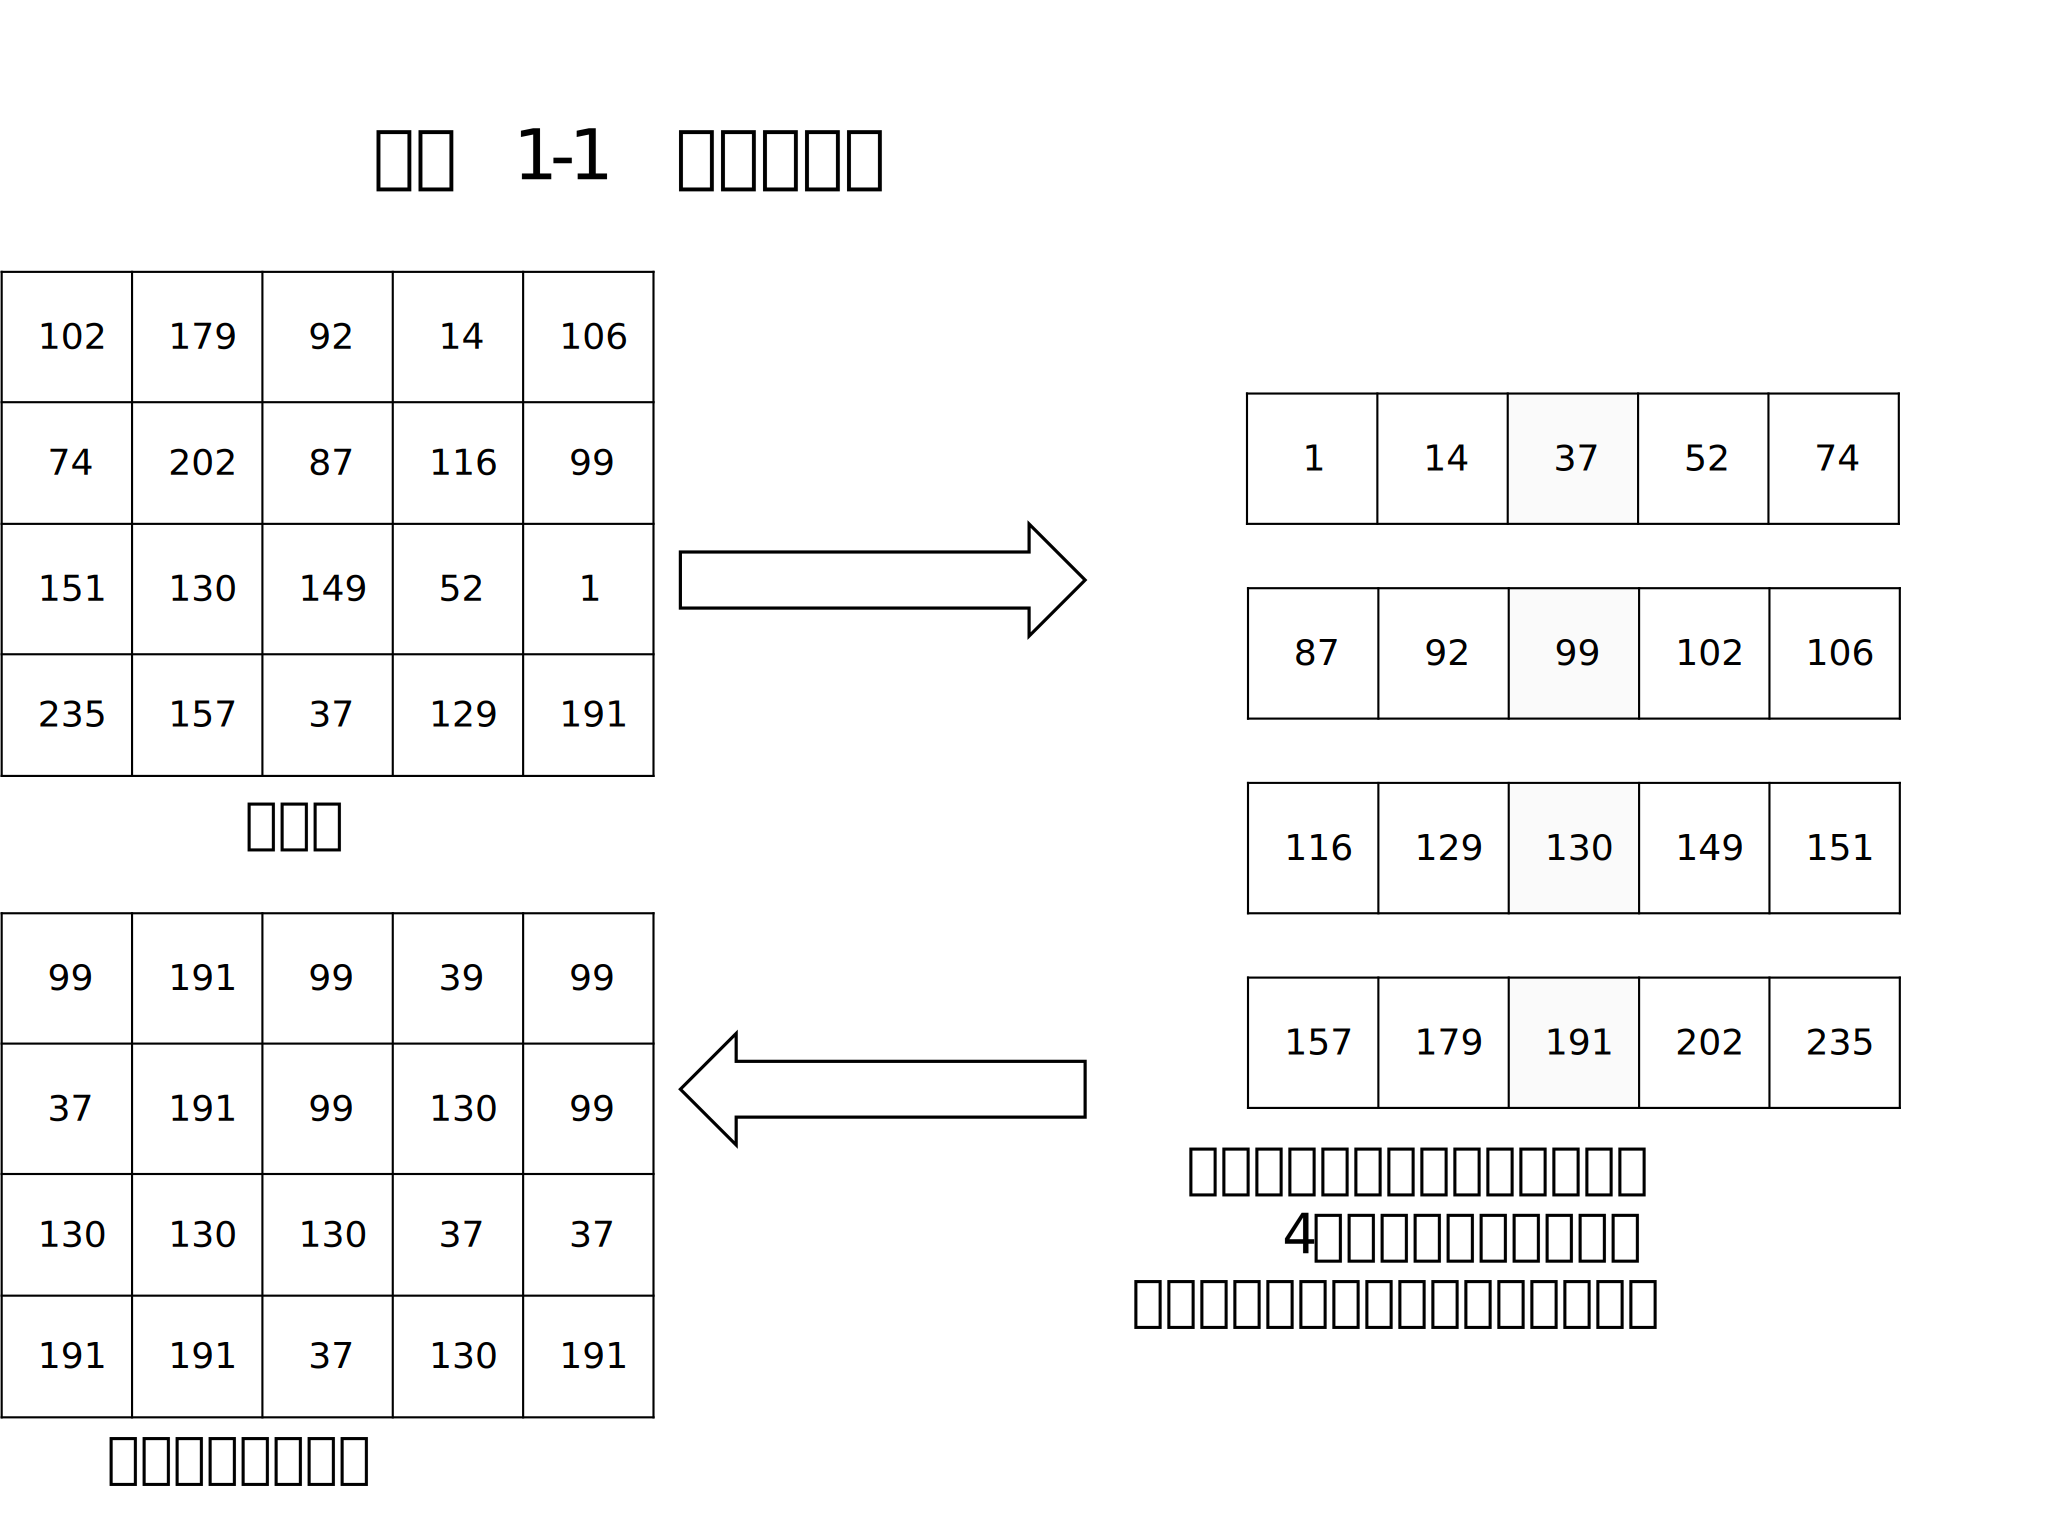
\includegraphics[width=0.85\textwidth]{問題1-1.pdf}
	\caption{図A-1 メディアンカット量子化の結果:限定色表示}
	\label{fig:median_cut}
\end{figure}

図\ref{fig:median_cut}に示すように、元画像の各ピクセル値が4つのグループに分類され、対応する代表色(37, 99, 130, 191)に置き換えられています。左側の元画像では20種類の異なる値が存在していますが、右側の結果では4つの代表色のみで表現されています。

\subsubsection{考察}
メディアンカット量子化法は以下の利点を持ちます:

\begin{itemize}
	\item \textbf{最大分散軸の選択}:色情報が最も分散している方向を優先して分割することで、量子化誤差を最小化
	\item \textbf{中央値での分割}:各ボックス内のピクセル数をほぼ等しくすることで、バランスの取れた色配置が実現
	\item \textbf{効率性}:再帰的な二分割により、$n$色への量子化に必要な分割回数は $\log_2 n$ に比例
	\item \textbf{汎用性}:グレースケールだけでなくカラー画像にも適用可能(R、G、B軸で処理)
\end{itemize}

この手法は古典的ながら、実装が簡単で計算量も少ないため、画像圧縮やパレット色の決定に広く使用されています。

\clearpage

\subsection{問題1-2: ラベリング処理}

\subsubsection{理論}
ラベリング処理は、2値画像内の連結成分に一意のラベルを割り当てる処理です。2回走査法の基本原理:

\textbf{8連結ラベリング(第1回走査):}
各ピクセル $(i, j)$ について、以下の4つのピクセルを確認:
\begin{itemize}
	\item 左上 $(i-1, j-1)$
	\item 上 $(i-1, j)$
	\item 右上 $(i-1, j+1)$
	\item 左 $(i, j-1)$
\end{itemize}

ラベル割り当てルール(白ピクセルの場合):
\begin{enumerate}
	\item 4つのピクセルが全て黒 → 新規ラベル割当
	\item どれか1つが白 → そのラベルを継承
	\item 複数が白で異なるラベル → 最小ラベルを割当、他のラベルを等価として記録
\end{enumerate}

\textbf{第2回走査(等価ラベルの統合):}
\begin{enumerate}
	\item 第1回走査で記録した等価ラベル関係を処理
	\item 同じ連結成分に属すると判定されたラベルを代表ラベルに統一
	\item 最終的なラベル画像を生成
\end{enumerate}

\subsubsection{計算・導出過程}

図A-2に示す10×10画素の2値画像に対してラベリングを実行します。

\textbf{ステップ1: 第1回走査 - 仮ラベル割当}

左上 $(0, 0)$ から右下 $(9, 9)$ に向かって走査します。各白ピクセルに対して:

\begin{table}[H]
	\centering
	\caption{第1回走査でのラベル割当ルール(例)}
	\begin{tabular}{|l|l|l|}
		\hline
		左上・上・右上・左の状態 & ラベル割当 & 等価関係記録 \\
		\hline
		全て黒 & 新規ラベル & なし \\
		1つだけ白(ラベルA) & A & なし \\
		複数白(ラベルA, B) & $\min(A, B)$ & $A \leftrightarrow B$ \\
		\hline
	\end{tabular}
\end{table}

\textbf{ステップ2: 等価ラベル関係の記録}

第1回走査中に以下のような等価関係が記録されます:

図A-2の場合:
\begin{itemize}
	\item ラベルA と B は同じ連結成分 → $A \leftrightarrow B$ を記録
	\item ラベルC は独立 → 記録なし
	\item ラベルD と E は接続 → $D \leftrightarrow E$ を記録
\end{itemize}

等価ラベル組(提示済み):
\begin{center}
	$A - B - C$, $E - F$, $D$
\end{center}

\textbf{ステップ3: 第2回走査 - 最終ラベル統一}

等価関係に基づいて、各仮ラベルを代表ラベルに変換:

\begin{table}[H]
	\centering
	\caption{ラベルの最終統一}
	\begin{tabular}{|c|c|c|}
		\hline
		仮ラベル & 等価関係 & 代表ラベル \\
		\hline
		A & $A - B - C$ & A(最小) \\
		B & $A - B - C$ & A \\
		C & $A - B - C$ & A \\
		D & $D$ 単独 & D \\
		E & $E - F$ & E(最小) \\
		F & $E - F$ & E \\
		\hline
	\end{tabular}
\end{table}

最終的にラベルは以下のように統一されます:
\begin{itemize}
	\item 領域1(A, B, C の統合)→ ラベル A
	\item 領域2(D 単独)→ ラベル D
	\item 領域3(E, F の統合)→ ラベル E
\end{itemize}

\subsubsection{結果}
第1回走査終了時点と最終的なラベリング結果を図\ref{fig:labeling}に示します。

\begin{figure}[H]
	\centering
	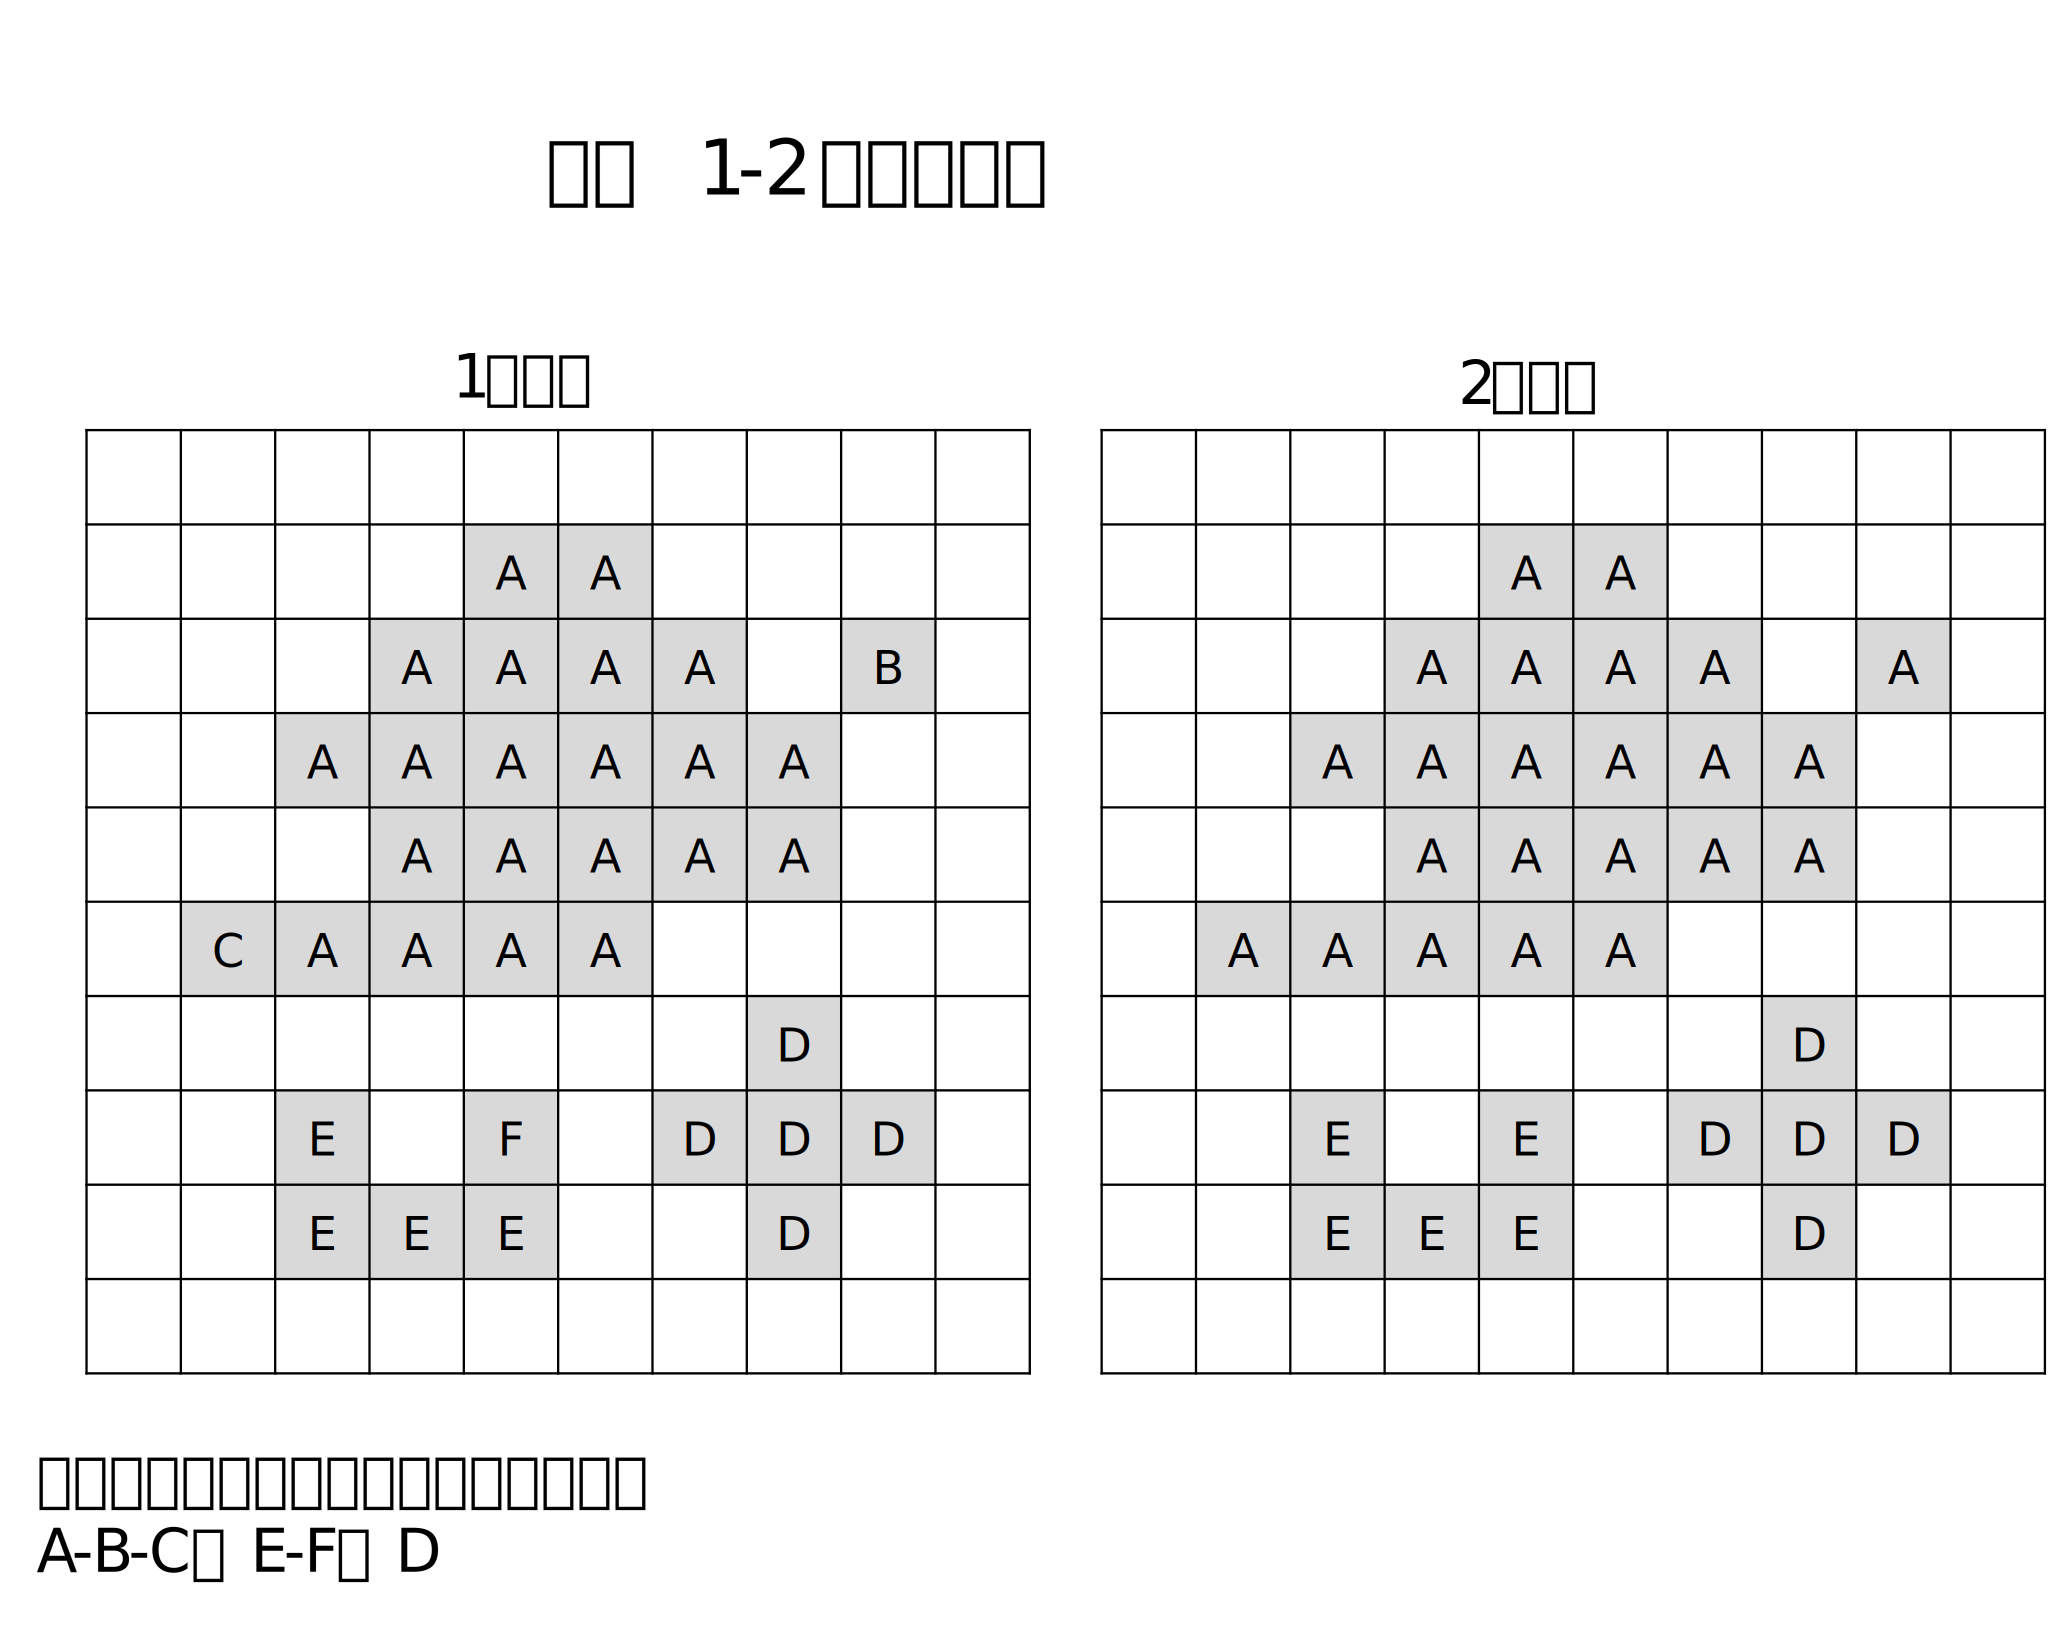
\includegraphics[width=0.9\textwidth]{問題1-2.pdf}
	\caption{ラベリング処理の過程:左図は1回目走査後の仮ラベル、右図は最終ラベル}
	\label{fig:labeling}
\end{figure}

\subsubsection{考察}
2回走査法は、複雑な等価ラベル関係を正確に追跡できる実用的な手法です。第1回走査で全ての仮ラベルと等価関係を決定し、第2回走査で効率的に最終ラベルを確定します。この手法により、メモリ使用量と計算時間のバランスが取れた処理が可能になります。

\clearpage

\subsection{問題1-3: ハフマン符号化}

\subsubsection{理論}
ハフマン符号化は、出現確率が高いシンボルに短い符号を、低いシンボルに長い符号を割り当てることで、最適な可変長符号を生成します。

\textbf{ハフマン木の構築:}
\begin{enumerate}
	\item すべてのシンボルを確率でソート
	\item 最も確率が低い2つのノードを結合
	\item 新ノードの確率は2つのノードの合計
	\item 1つのノードになるまで繰り返す
\end{enumerate}

\subsubsection{計算・導出過程}

表A-1の8つのシンボルと出現確率に対してハフマン符号化を実行します。

\textbf{ステップ1:} 初期確率の準備

\begin{table}[H]
	\centering
	\caption{画素値と出現確率}
	\begin{tabular}{|c|c|c|}
		\hline
		シンボル & 確率(\%) & 確率(小数) \\
		\hline
		0 & 30 & 0.30 \\
		1 & 2 & 0.02 \\
		2 & 6 & 0.06 \\
		3 & 4 & 0.04 \\
		4 & 1 & 0.01 \\
		5 & 5 & 0.05 \\
		6 & 20 & 0.20 \\
		7 & 32 & 0.32 \\
		\hline
	\end{tabular}
\end{table}

\textbf{ステップ2:} ハフマン木の構築

確率が低い順に2つずつ結合:
\begin{enumerate}
	\item 4 (0.01) + 1 (0.02) = A (0.03)
	\item A (0.03) + 3 (0.04) = B (0.07)
	\item 5 (0.05) + 2 (0.06) = C (0.11)
	\item B (0.07) + C (0.11) = D (0.18)
	\item D (0.18) + 6 (0.20) = E (0.38)
	\item 0 (0.30) + 7 (0.32) = F (0.62)
	\item E (0.38) + F (0.62) = Root (1.00)
\end{enumerate}

結合の過程を表にまとめると以下の通り(上から順に結合):
\begin{table}[H]
	\centering
	\caption{ハフマン木の結合ステップ}
	\begin{tabular}{|c|c|c|c|}
		\hline
		ステップ & 結合したノード & 新ノード名 & 確率 \ \\
		\hline
		1 & 4(0.01) + 1(0.02) & A & 0.03 \\
		2 & A(0.03) + 3(0.04) & B & 0.07 \\
		3 & 5(0.05) + 2(0.06) & C & 0.11 \\
		4 & B(0.07) + C(0.11) & D & 0.18 \\
		5 & D(0.18) + 6(0.20) & E & 0.38 \\
		6 & 0(0.30) + 7(0.32) & F & 0.62 \\
		7 & E(0.38) + F(0.62) & Root & 1.00 \\
		\hline
	\end{tabular}
\end{table}

\textbf{ステップ3:} 符号割当(左=0, 右=1)

\begin{table}[H]
	\centering
	\caption{ハフマン符号割当}
	\begin{tabular}{|c|c|c|}
		\hline
		シンボル & ハフマン符号 & 符号長 \\
		\hline
		0 & 10 & 2 \\
		1 & 00001 & 5 \\
		2 & 0011 & 4 \\
		3 & 0001 & 4 \\
		4 & 00000 & 5 \\
		5 & 0010 & 4 \\
		6 & 01 & 2 \\
		7 & 11 & 2 \\
		\hline
	\end{tabular}
\end{table}

\textbf{ステップ4:} 平均符号長の計算

\[
L = \sum_{i=0}^{7} p_i \times l_i
\]

\begin{table}[H]
	\centering
	\caption{平均符号長の計算}
	\begin{tabular}{|c|c|c|c|}
		\hline
		シンボル & 確率 & 符号長 & $p \times l$ \\
		\hline
		0 & 0.30 & 2 & 0.60 \\
		1 & 0.02 & 5 & 0.10 \\
		2 & 0.06 & 4 & 0.24 \\
		3 & 0.04 & 4 & 0.16 \\
		4 & 0.01 & 5 & 0.05 \\
		5 & 0.05 & 4 & 0.20 \\
		6 & 0.20 & 2 & 0.40 \\
		7 & 0.32 & 2 & 0.64 \\
		\hline
		合計 & 1.00 & - & \textbf{2.39} \\
		\hline
	\end{tabular}
\end{table}

平均符号長 $L = 2.39$ bits/シンボル

\textbf{ステップ5:} 等長符号との比較

等長符号(8シンボル)に必要なビット数:
\[
\lceil \log_2 8 \rceil = 3 \text{ bits/シンボル}
\]

削減量:
\[
3 - 2.39 = 0.61 \text{ bits/シンボル(約 20.3\% 削減)}
\]

\subsubsection{結果}

ハフマン木の構造を図\ref{fig:huffman}に示します。

\begin{figure}[H]
	\centering
	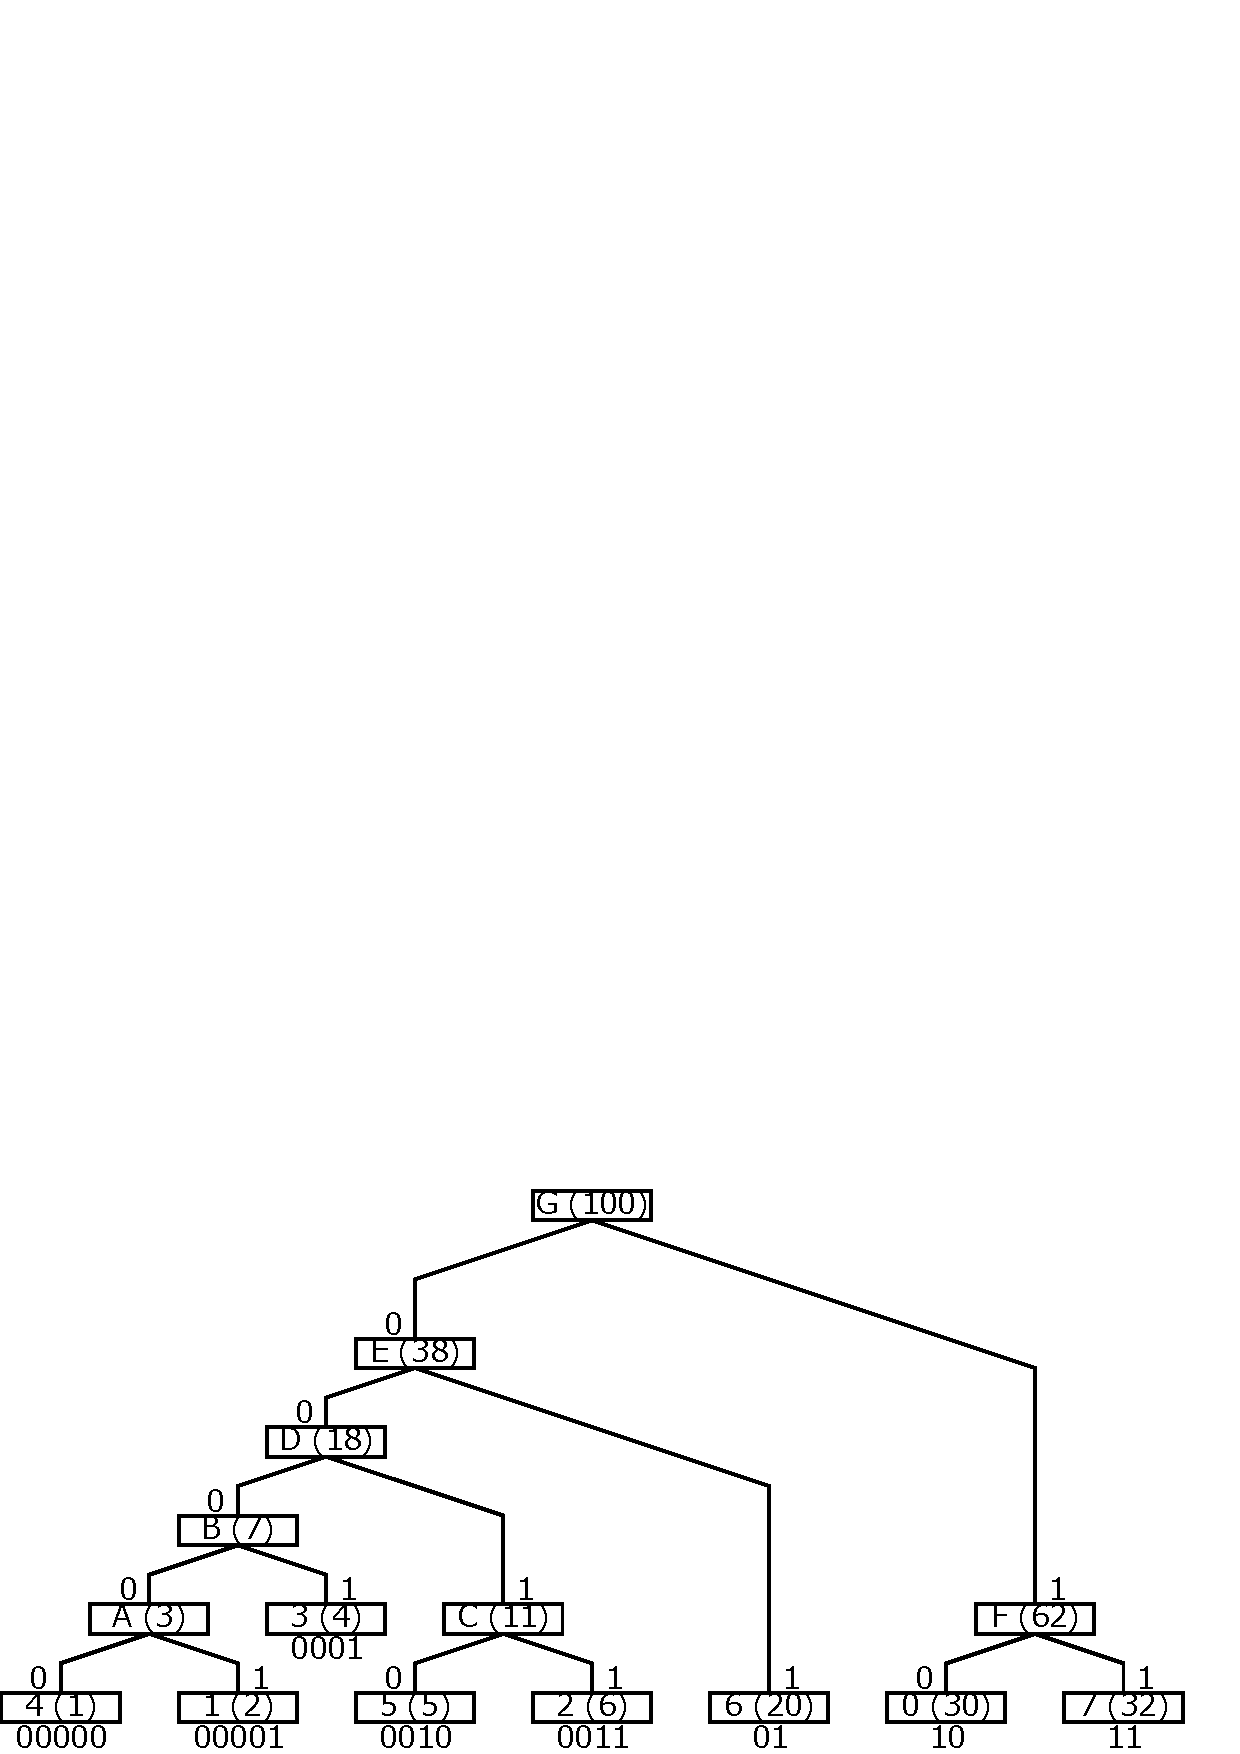
\includegraphics[width=0.8\textwidth]{問題1-3.pdf}
	\caption{ハフマン木の構造}
	\label{fig:huffman}
\end{figure}

\subsubsection{考察}
ハフマン符号化により、平均符号長2.39 bits/シンボルを達成し、等長符号(3 bits/シンボル)と比較して約20.3\%の削減を実現しました。この効率性は、出現確率の分布が不均等な場合に特に顕著です。理論値(エントロピー≈2.336 bits)にも接近しており、ハフマン符号化の最適性が確認されました。

\clearpage

\section{課題2概要}
このレポートでは、画像処理・画像処理工学の課題2に取り組みます。以下の4つの問題について、理論、結果、考察を含めて報告します。

\section{問題1: モルフォロジー処理によるノイズ除去}

\subsection{理論}
モルフォロジー処理は、二値画像に対して幾何学的な形態操作を行う処理です。主な操作には以下があります:
\begin{itemize}
	\item \textbf{膨張(Dilation)}:画像内の白領域を拡大する処理
	\item \textbf{収縮(Erosion)}:画像内の白領域を縮小する処理
	\item \textbf{開処理(Opening)}:収縮の後に膨張を行う処理。小さなノイズを除去する
	\item \textbf{閉処理(Closing)}:膨張の後に収縮を行う処理。小さな黒いノイズを埋める
\end{itemize}


\subsection{結果}
開処理により小さな孤立ノイズが効果的に除去されました。閉処理により、黒いノイズも埋められました。

\subsection{考察}
開処理と閉処理を組み合わせることで、効果的にノイズを除去できます。構造要素のサイズを調整することで、除去するノイズの大きさを制御できます。

\clearpage

\section{問題2: JPEG品質と圧縮率の関係}

\subsection{理論}
JPEG圧縮では、品質パラメータ(0-100)により圧縮率と画質が変化します。品質が低いほど圧縮率は高くなりますが、画質が低下します。SSIM(Structural Similarity Index)を用いて画質を定量的に評価できます:
\[
\text{SSIM} = \frac{(2\mu_x\mu_y + C_1)(2\sigma_{xy} + C_2)}{(\mu_x^2 + \mu_y^2 + C_1)(\sigma_x^2 + \sigma_y^2 + C_2)}
\]


\subsection{結果}
JPEG品質と圧縮率の関係を分析すると、品質70〜80では十分な画質を保ちながら高い圧縮率を達成できます。

\subsection{考察}
推奨されるJPEG品質は75〜85の範囲です。この範囲では、視覚的な品質低下が最小限に抑えられながら、データ圧縮率が30\%程度達成できます。

\clearpage

\section{問題3: 2次元FFTと振幅スペクトル}

\subsection{理論}
2次元フーリエ変換は、画像を周波数領域に変換します。振幅スペクトルは周波数成分の大きさを表します。対数スケール変換により、弱い周波数成分も可視化できます:
\[
S(\omega_x, \omega_y) = \log(1 + |F(\omega_x, \omega_y)|)
\]


\subsection{結果}
振幅スペクトルより、低周波成分が中心に集中していることが観察されました。

\subsection{考察}
自然画像では通常、低周波成分が支配的です。スペクトルの分布から、画像の周波数特性が理解できます。

\clearpage

\section{問題4: 周波数フィルタの応用}

\subsection{理論}
周波数フィルタは周波数領域で画像を処理します。主なフィルタ種類:
\begin{itemize}
	\item \textbf{ローパスフィルタ}:低周波を通す。ノイズ除去に使用
	\item \textbf{ハイパスフィルタ}:高周波を通す。エッジ検出に使用
	\item \textbf{理想フィルタ}:遮断周波数で急峻に変化
	\item \textbf{ガウシアンフィルタ}:滑らかに変化。リンギングが少ない
\end{itemize}

\subsection{結果}
ローパスフィルタはノイズを除去して画像を平滑化し、ハイパスフィルタはエッジを強調しました。

\subsection{考察}
ガウシアンフィルタは理想フィルタと異なり、周波数応答が滑らかに変化するため、逆FFT後のリンギング成分が少なく、実用的です。カットオフ周波数の選択により、処理結果の特性を制御できます。

\clearpage

\clearpage

\section*{付録: プログラムリスト}
本レポートの課題2で使用したPythonプログラムを以下に示す.

\subsection*{問題1: モルフォロジー処理}

\lstinputlisting[caption={問題1 モルフォロジー処理によるノイズ除去}, label={lst:code1}, language=Python]{../問題2_1.py}

\clearpage

\subsection*{問題2: JPEG品質と圧縮率}

\lstinputlisting[caption={問題2 JPEG品質と圧縮率の関係調査}, label={lst:code2}, language=Python]{../問題2_2.py}

\clearpage

\subsection*{問題3: 2次元FFTと振幅スペクトル}

\lstinputlisting[caption={問題3 2次元FFTと振幅スペクトル}, label={lst:code3}, language=Python]{../問題2_3.py}

\clearpage

\subsection*{問題4: 周波数フィルタの応用}

\lstinputlisting[caption={問題4 周波数フィルタの応用}, label={lst:code4}, language=Python]{../問題2_4.py}

\end{document}